\section{Experiences and Numerical Analysis}

\subsection{Analysis of the ascent step convergence}
\label{sec:ascent_convergence}
 During the iterative procedure, we plot in Figure \ref{fig:ascent_criteria} the evolution of the norm of the gradient of $F$, for $j \in \intinter{1}{J}$. The stochastic ascent gradient seems to converge as the norm of the gradient reaches a plateau. The convergence is faster for the 2D discrete distributions than for the 1D continuous distributions. 

 \begin{figure}
    \begin{subfigure}{.5\textwidth}
        \centering
        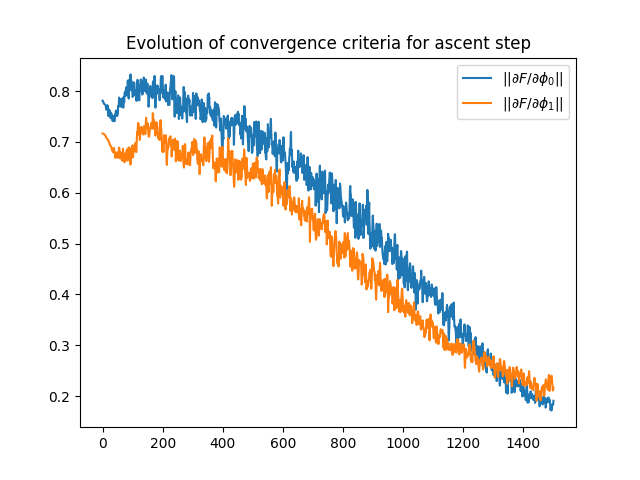
\includegraphics[width=\textwidth]{figures/ascent_criteria_msamples16000_iter0_1D_2skewnorm.png}
        \caption{Two 1D continuous distributions}
    \end{subfigure}
    \begin{subfigure}{.5\textwidth}
        \centering
        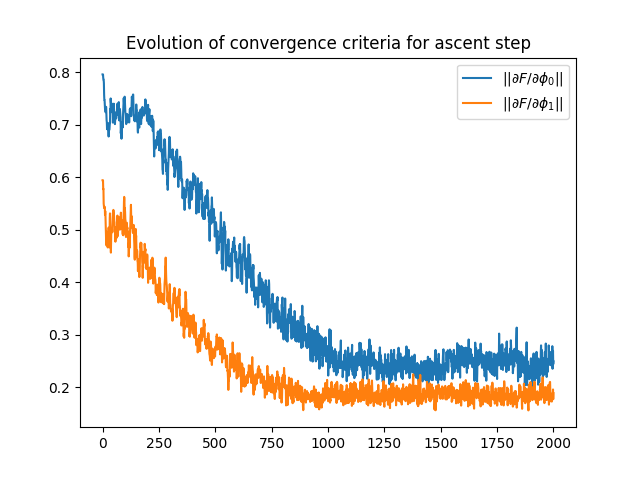
\includegraphics[width=\textwidth]{figures/ascent_criteria_msamples16000_iter0_2D_discrete.png}
        \caption{Two 2D discrete distributions }
    \end{subfigure}
    \caption{Evolution of $\norm{ \frac{\partial F}{\partial \phi_j} }$ during the ascent step (Algorithm \ref{ascent}) for each experiment. In the x-axis, is the number of interations of the while loop.}
    \label{fig:ascent_criteria}
\end{figure}

It is worth noting that the majority of the computation time is consumed by the ascent step (several hours) as shown in Table \ref{table:time_algo_table}.

In \cite{claici_stochastic_2018}, the authors use a step size of $\alpha = 10^{-3}$ and a stop criteria of $\epsilon_{ascent} = 10^{-6}$ in Algorithm \ref{ascent}. However, the while loop took an excessive amount of time to converge, exceeding $6$ hours. To enhance computational efficiency, we opt for $\alpha = 0.05$ and $\epsilon_{ascent} = 10^{-4}$. Nesterov acceleration is set to $\beta = 0.99$ like in \cite{claici_stochastic_2018}. Additionally, we introduce a maximum number of iterations, limiting the while loop to $T_{max} = 1500$ for efficiency. 

We employ a single iteration for both of our experiments, as the authors \cite{claici_stochastic_2018} assert that the entire algorithm converges within a single iteration.

\begin{table}
    \begin{center}
            \begin{tabular}{lrr}
                    Experiment & Ascent step & Snap step \\
                    \hline\hline
                    1D skewnorm & $8309.44 \pm 0.33$ & $5.28 \pm 0.23$ \\
                    2D discrete & $11938.70 \pm 0.34$ & $9.81 \pm 0.34$ \\
            \end{tabular}
    \end{center}
    \caption{Computation time (in seconds) for each step of the Algorithm \ref{ascent_snap}. The experiences are repeated $3$ times.}
    \label{table:time_algo_table}
\end{table}

\subsection{Quantitative Analysis and Comparative Evaluation}

\subsubsection{Optimal Monge Map Approach to Barycenter Computation}
\label{sec:monge_map}

In the case $\mathcal{X} = \mathcal{Y} = \RR^d$ and $d(x, y)^2 = \norm{x  - y}^2$ and if at least one of the two input measures has a density with respect to the Lebesgue measure, the Theorem $2.1$ of \cite{peyre_computational_2020} states that the optimal coupling $\pi$ of \eqref{eq:W2} is unique and is given by $\pi = (Id, T)_\#\mu$ where $T : \mathcal{X} \rightarrow \mathcal{Y}$ denote the "optimal Monge map" with $T_\#\mu = \nu$. 

In the 1D case \cite[see][Remark 2.30]{peyre_computational_2020}, $d=1$, the optimal Monge map between two distributions $\mu_1$ and $\mu_2$ writes 

\begin{equation}\label{eq:monge_map}
    T=\mathcal{C}^{-1}_{\mu_2}\ o\ \mathcal{C}_{\mu_1} 
\end{equation}

where $\mathcal{C}_{\mu} : \RR \rightarrow [0, 1]$ and $\mathcal{C}^{-1}_\mu : [0, 1]\rightarrow \RR $ are respectively the cumulative distribution function and its pseudoinverse, also called the generalized quantile function of $\mu$ .

Using the Remark $7.1$ \cite{peyre_computational_2020}, the McCann's interpolation \cite{mccann_convexity_1997} between two measures reads, for $t\in [0, 1]$ 
\begin{align}
    \mu_t &= (tT + (1-t)Id)_\#\mu_1 \nonumber \\
    \mu_t &= (t\mathcal{C}^{-1}_{\mu_2}\ o\ \mathcal{C}_{\mu_1} + (1-t)Id)_\#\mu_1 \label{eq:mccann}
\end{align}

Figure \ref{fig:mccann_1D_2skew} shows the displacement interpolation between 1D measures, using the cumulative distribution function as detailed in \eqref{eq:mccann}.

\begin{figure}
    \centering
    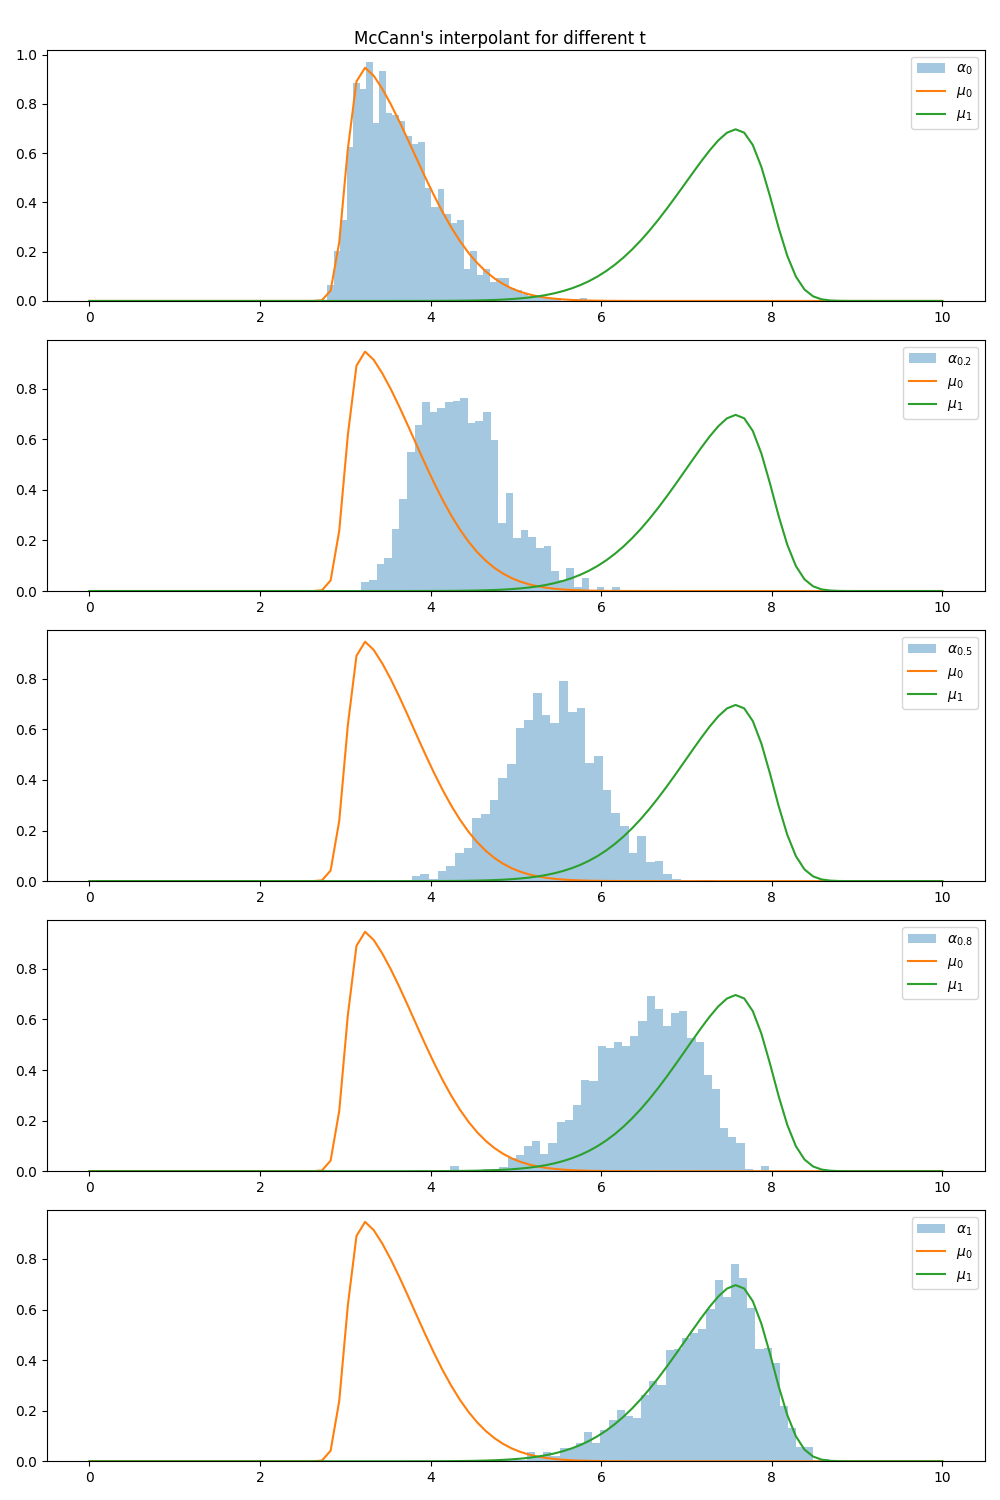
\includegraphics[width=\textwidth]{figures/mccann_1D_2skew.png}
    \caption{McCann's interpolant between two skew-normal distributions. From top to bottom, $t$=0, 0.2, 0.5, 0.8, 1. The barycenter that we will consider corresponds to $t=0.5$, depicted in the middle plot.}
    \label{fig:mccann_1D_2skew}
\end{figure}

To obtain the interpolant, we generate $K$ samples $(X_k)$ independent and identically distributed (iid) according to $\mu_1$. Then, we compute the samples $(Y_k)$ as follows 
$$Y_k = tT X_k + (1-t)X_k, \qquad \forall k \in\intinter{1}{K}$$ 
where $T$ is given in \eqref{eq:monge_map}. We have that $ (Y_k)$ is iid according to $\mu_t$.

To compare with the algorithm \ref{ascent_snap}, we use $t=0.5$. The only hyperparameter to fix is the number of samples $K$ to generate. We choose $K=2000$. The inconvenient is that we can apply this computation only in the 1D case and for two input measures.

\subsubsection{Use of the Sinkhorn algorithm to compute the barycenter} \label{sec:iterative_bregman}

We will also compare our algorithm \ref{ascent_snap} to the computation of the barycenter using the Sinkhorn algorithm \cite{peyre_computational_2020}. This algorithm solved the discretized regurlarized optimal transport problem using the optimality condition that shows that the optimal coupling $P_\epsilon$ necessarily has the form 
$$P_\epsilon = diag\left(u\right) K\ diag\left(v\right)$$
where the Gibbs kernel is defined as
$$K := e^{-\frac{C}{\epsilon}}.$$
where $C_{ij} = d(x_i, y_j)^2$ is the cost matrix. The vectors $u$ and $v$ are non negative vectors. $\epsilon$ is the regularization parameter.

Figure \ref{fig:sinkhorn_1D_2skew} depicts the barycenter obtained for various $\epsilon$. It's worth noting that the algorithm encounters instability issues for $\epsilon$ values below $0.005$. As illustrated, the lower $\epsilon$, the sharper the density of the barycenter.

\begin{figure}
    \centering
    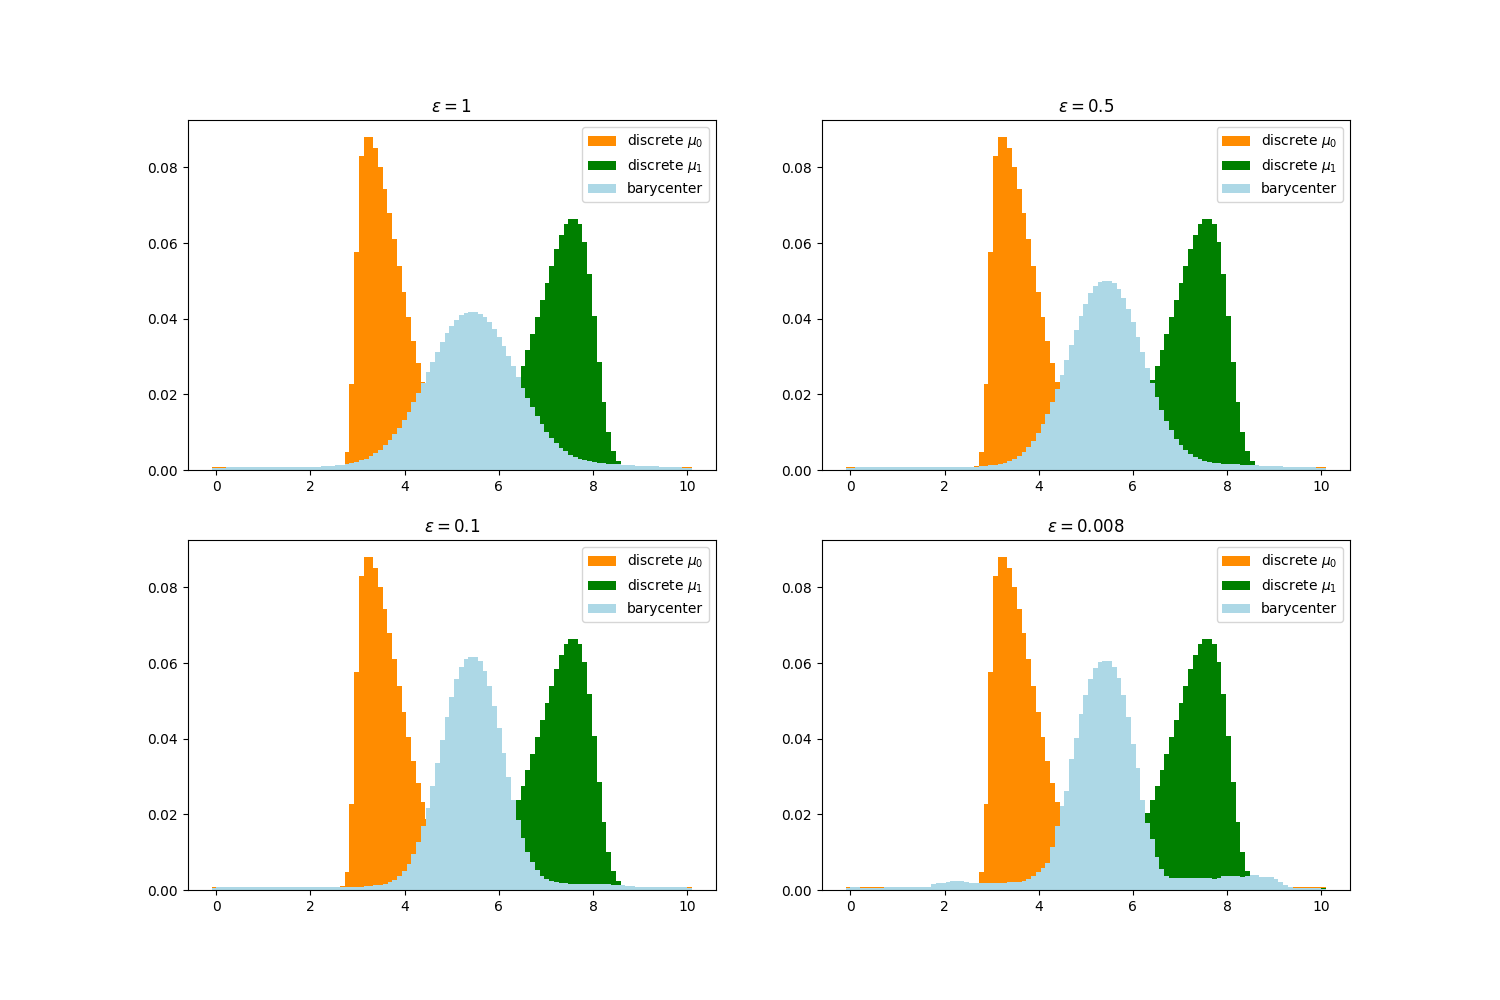
\includegraphics[width=\textwidth]{figures/sinkhorn_1D_2skew.png}
    \caption{Histogram showing the input distributions (skew-normal distributions) and the barycenter computed using the Sinkhorn algorithm for different values of the regurlarized parameter $\epsilon$.}
    \label{fig:sinkhorn_1D_2skew}
\end{figure}

In our experiments, we use $500$ iterations and we fix $\epsilon = 0.01$ for the $1D$ case and $\epsilon = 0.04^2$ for the $2D$ case. 

\begin{figure}
    \centering
    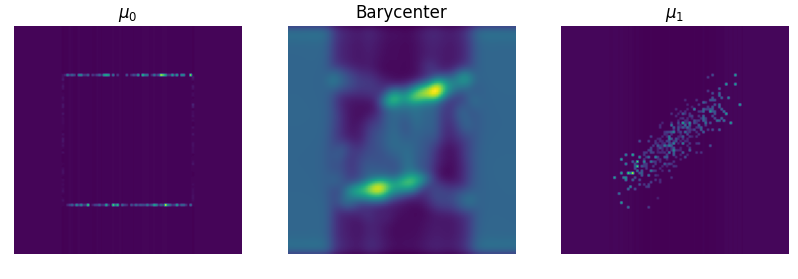
\includegraphics[width=\textwidth]{figures/sinkhorn_barycenter_2D_discrete.png}
    \caption{Results of the Sinkhorn algorithm for the 2D discrete case. The regularization is $\epsilon = 0.04^2$.}
    \label{fig:sinkhorn_2D_discrete}
\end{figure}

\subsubsection{A free grid Sinkhorn algorithm approach from POT toolbox}
\label{sec:pot}

The POT toolbox (Python Optimal Transport) \cite{flamary_pot_2021} contains implementations of a number of founding works of OT for machine learning such as Sinkhorn algorithm and Wasserstein barycenters. In particular, it provides an algorithm\footnote{\url{https://pythonot.github.io/gen_modules/ot.bregman.html_\#ot.bregman.free_support_sinkhorn_barycenter}} based on \cite{cuturi_fast_2014} (Algorithm 2) that solves the free support regularized Wasserstein barycenter problem. Like the method \S\ref{sec:method}, we optimize over the locations of the barycenter but not over its weights. 

The figures \ref{pot1}, \ref{pot2} and \ref{pot3} in the Appendices shows the influence of the regularization $\epsilon$ on the free support barycenters for the 2D dataset.

\begin{figure}
    \centering
    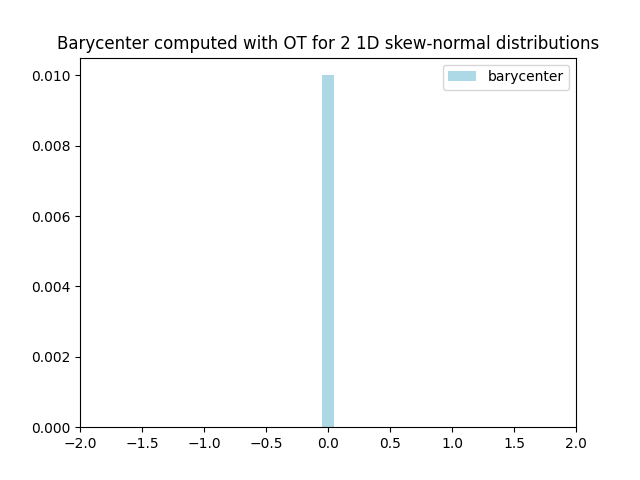
\includegraphics[scale=.4]{figures/ot_barycenter_1D_2skewnorm.png}
    \caption{Results of the POT toolbox for the 1D continuous case. }
    \label{fig:pot_1D_2skewnorm}
\end{figure}

\subsubsection{Experience 1 : 1D skewed normal distributions}

In this experience, we compute the barycenter between two 1D skewed normal distributions whose skew parameters are $s_1=8$ and $s_2=4$, means are $m_1=3$ and $m=8$ and standart deviations are $\sigma_1=0.8$ and $\sigma_2=1$, respectively.  

The figures \ref{fig:mccann_1D_2skew}, \ref{fig:pot_1D_2skewnorm}, \ref{fig:ascent_snap_1D_2skewnorm} and \ref{fig:sinkhorn_1D_2skew} depict the results for each methods. The support of the barycenter computed by the proposed method is larger than the support of the McCann's interpolation and the one obtained with the Sinkhorn algorithm. 

Moreover, uniform weights does not seem to be a good way to approximate barycenters of non-uniform distributions.

\begin{figure}
    \centering
    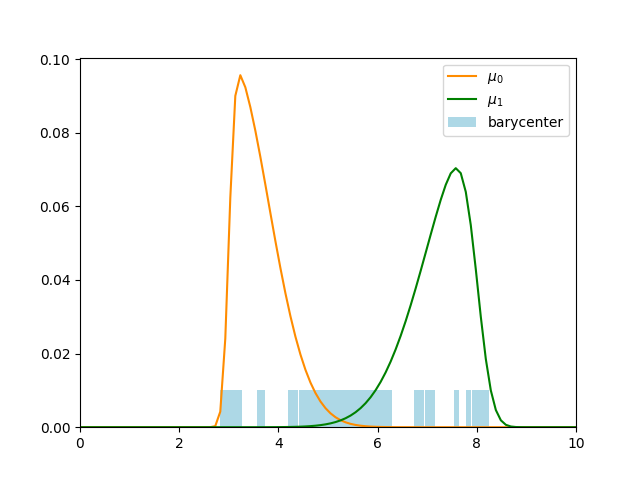
\includegraphics[width=\textwidth]{figures/ascent_snap_1D_2skewnorm.png}
    \caption{Results of the ascent/snap Algorithm \ref{ascent_snap} for the 1D continuous case. We use $16000$ samples from the input distributions, and $1$ iterations. See Section \ref{sec:ascent_convergence} for the hyperparameters.}
    \label{fig:ascent_snap_1D_2skewnorm}
\end{figure}

Running the free support sinkhorn algorithm from the POT toolbox did not yield any results as can be see on the Figure \ref{fig:pot_1D_2skewnorm}.

Regarding the computation time, the ascent/snap algorithm is by far the slowest algorithm. The table \ref{table:time_table} shows the computation time for each method in each test case.

\subsubsection{Experience 2 : 2D uniform distributions}

In the second experiment, we generate two 2D uniform distributions. We generate $160$ points from each distribution with a different geometrical structures. The first distribution is a square and the points from the second distribution are generated from a multivariate normal distribution with mean $(0, 0)$ and covariance matrix
$
\Sigma = \left(\begin{array}{cc}
0.6 & 0.5 \\
0.5 & 0.6
\end{array}\right)
$.

\begin{figure}
    \centering
    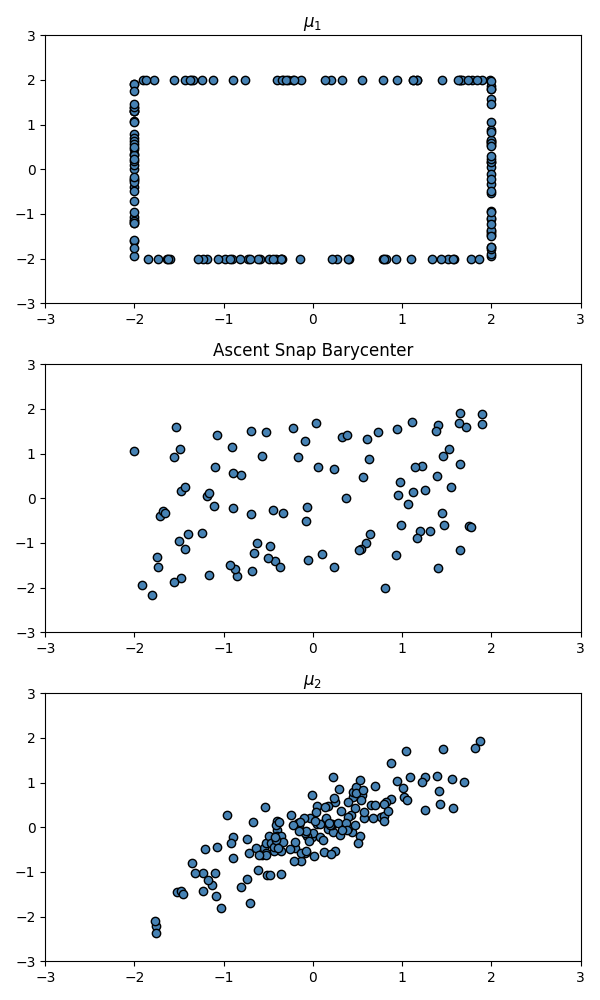
\includegraphics[width=\textwidth]{figures/ascent_snap_2D_discrete_barycenter.png}
    \caption{Results of the ascent/snap Algorithm \ref{ascent_snap} for the 2D discrete case. We use $16000$ samples from the input distributions, and $1$ iteration.}
    \label{fig:ascent_snap_2D_discrete}
\end{figure}

The barycenter computed by the proposed method showed in Figure \ref{fig:ascent_snap_2D_discrete} is slightly different from the one obtained with the free support Sinkhorn algorithm from POT \S\ref{sec:pot}. Our algorithm gives point inside the warped square whereas the POT barycenter only warped the segments. However, their shapes are similar. 

As illustrated in The Figure \ref{fig:sinkhorn_2D_discrete}, we had to construct an image to apply the Sinkhorn algorithm to 2D distributions corresponding to this scheme. However, this algorithm do not yield qualitative results as the Gibbs kernel tend to smooth the image.

\begin{table}
    \begin{center}
        \begin{tabularx}{\textwidth}{>{\raggedright}m{2cm} c m{2cm} X X}
                Experiment & McCann & Iterative Bregman & POT free support & Ascent Snap \\
                \hline\hline
                1D skewnorm & $0.02 \pm 0.01$ & $0.22 \pm 0.02$ & $0.74 \pm 0.28$ & $7814.27 \pm 0.37$ \\
                2D discrete & - & $2.18 \pm 0.34$ & $0.38 \pm 0.30$ & $16351.66 \pm 0.23$ \\
        \end{tabularx}
    \end{center}
    \caption{Computation time (in seconds) for the different methods}
    \label{table:time_table}
\end{table}



